\documentclass[10pt]{article}
\usepackage{../local}
\usepackage{mathrsfs}
\newcommand{\laplace}{\nabla^2}

\newcommand{\classcode}{Physics 110A}
\newcommand{\classname}{Electrodynamics and Optics}
\renewcommand{\maketitle}{%
\hrule height4pt
\large{Eric Du \hfill \classcode}
\newline
\large{HW 05} \Large{\hfill \classname \hfill} \large{\today}
\hrule height4pt \vskip .7em
\normalsize
}
\linespread{1.1}
\begin{document}
	\maketitle
	\section*{Collaborators}
	I worked with \textbf{Teja Nivarthi, Nathan Song, Andrew Binder, Christine Zhang} and \textbf{Nikhil 
	maserang} to complete this assignment.

	\section*{Problem 1}

	Suppose we have a charge distribution $\rho_1(r)$ and a potential $V_2(r)$. The potential energy of this 
	system is given by 
	\[
		\int_{\text{all space}} \rho_1V_2 dr
	\] 
	Recall that for localized charge distributions, and with the boundary condition $V \to 0$ at infinity, one
	can write the potential created by a charge distribution as
	\[
	V = \frac{1}{4\pi \epsilon_0}\int \frac{\rho(\mathbf r')}{\rcurs} d\tau'
	\] 
	Show that the potential energy $\rho_1$ in the potential $V_2$ produced by $\rho_2$ is equal to the potential
	energy of $\rho_2$ in the potential $V_1$ produced by $\rho_1$. That is, 
	\[
		\int_{\text{all space}} \rho_1(\mathbf r) V_2(\mathbf r) d\tau =
		\int_{\text{all space}} \rho_2(\mathbf r')V_1(\mathbf r') d\tau'
	\] 
	This is called \textbf{Green's reciprocity relation}. In addition, using this relation, prove the ``\textit{
	mean value theorem}'' that we discussed in class: the average of $V(\mathbf r)$ over a spherical surface 
	$\mathcal S$ that encloses a charge-free volume is equal to the potential at the center of the sphere:
	\[
		\frac{1}{4\pi R^2}\int_{\mathcal S} V(\mathbf r) da = V(0)
	\] 

	\begin{solution}
		First, we rewrite the reciprocity relation in terms of the Laplacian:
		\[
			\int (\laplace V_1(r))V_2(r) d\tau = \int V_1(r')\laplace V_2(r') d\tau'
		\] 
		Now consider the left hand side of this equation:
		\[
		\int (\laplace V_1(r))V_2(r) d\tau
		\] 
		And now we use the relation that $\div(\grad V_1(r) V_2(r)) = \laplace V_1(r) V_2(r) + \grad V_1(r) 
		\grad V_2(r)$. Doing so, we get:
		\begin{align*}
			\int (\laplace V_1(r)) V_2(r) d\tau &=  \int \div(\nabla V_1(r) V_2(r)) - \int \nabla V_1(r) \nabla
			V_2(r)
		\end{align*}
		By the divergence theorem, the first term becomes $\int \div(\nabla V_1(r) V_2(r)) = \oint_{\partial V}
		\nabla V_1(r) V_2(r)$ and since we know that $V_2(r) = 0$ at infinity, this term vanishes. Computing the
		second term using integration by parts gets us:
		\begin{align*}
			-\int\nabla V_1(r) \nabla V_2(r) d\tau &= -\int \nabla(V_1(r) \nabla V_2(r)) -
			V_1(r) \laplace V_2(r) d\tau  \\
			&= \int V_1(r) \nabla^2V_2(r) d\tau
		\end{align*}
		which is equal to the right hand side. Notice also that integrating over all space is the same whether
		we are integrating over $r$ or $r'$ -- after all, we are still integrating the same system.

		To prove the mean value theorem, we consider two systems: one
		is the system we want to solve with charges outside generating potential $V_1$ (system 1),  and the
		other is a spherical shell with total surface
		charge $-Q = 4\pi R^2 \sigma$ and a positive charge $Q$ at the center (system 2). 
		
		In this second system, we have $V = 0$ outside the sphere because the potentials evenly cancel out. 
		Therefore outside the sphere,
		\[
		\int \rho_1V_2(r) d\tau = 0 \implies \int \rho_2(r) V_1(r) d\tau = 0
		\]
		We can write $\rho(r)$ as: 
		\[ \rho(r) = \frac{Q}{4\pi R^2} - Q\delta(0)\]
		The delta function here accounts for the fact that the charge is at the center of the sphere. Therefore: 
		\begin{align*}
			0 &=\int \left( \frac{Q}{4\pi R^2} - Q\delta(0)\right)V(r) \\
			\therefore \frac{Q}{4\pi R^2} \int_S V(r) &= Q \int V(r) \delta(0)\\
			\therefore \frac{1}{4\pi R^2} \int_S V(r) = V(0)
		\end{align*}
		I've skipped a lot of steps in this algebra because I couldn't type them up in time, but I believe this is the way to arrive at the proper conclusion.
	\end{solution}
	\pagebreak
	\section*{Problem 2}
	As shown in the right figure, we have a point charge $Q$ being placed in front of two semi-infinite 
	conducting plates that are perpendicular to each other, and are extended infinitely into the page, as well as
	to the right and to the left of the page. The line between the vertex and the charge form an angle $\alpha$
	with respect to the vertical plate. The conducting plates are grounded so that they have zero electric 
	potential. Find the net charge induced on each plate.
	
	\begin{solution}
		\begin{center}
			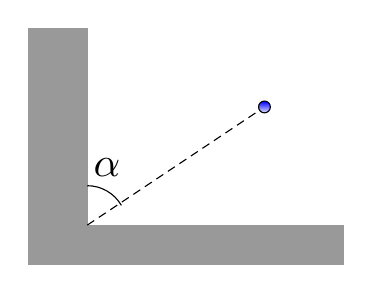
\begin{tikzpicture}
            \filldraw[gray!80] (0,0) -- (4,0) -- (4,0.5) -- (0.75,0.5) -- (0.75,3) -- (0,3) -- cycle;
            \draw[densely dashed] (0.75,0.5) -- (3,2);
            \draw[shading=axis, left color=blue, right color=blue!10!white, shading angle=0, anchor=center, fill opacity=1] (3,2) circle (0.075cm);
            \draw (0.75,1) arc (90:30:0.5cm) node[midway,above,scale=1.5] {$\alpha$};
			\end{tikzpicture}
		\end{center}
        Using the method of images, we have the following configuration (credit to Andrew for the Ti\textit kZ diagram)
        $$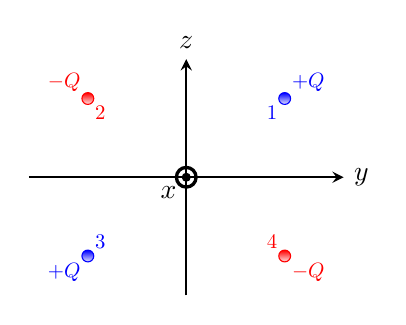
\begin{tikzpicture}
            \draw[thick, -stealth] (-2,0) -- (2,0) node[anchor=west] {$y$};
            \draw[thick, -stealth] (0,-1.5) -- (0,1.5) node[anchor=south] {$z$};
            \filldraw[black] (0,0) circle (0.05cm) node[anchor=north east] {$x$};
            \draw[very thick] (0,0) circle (0.125cm);
            \draw[blue, shading=axis, left color=blue, right color=blue!10!white, shading angle=0, anchor=center, fill opacity=1] (1.25,1) circle (0.075cm) node[anchor=south west, scale=0.75] {$+Q$} node[anchor=north east,scale=0.75] {$1$};
            \draw[blue, shading=axis, left color=blue, right color=blue!10!white, shading angle=0, anchor=center, fill opacity=1] (-1.25,-1) circle (0.075cm) node[anchor=north east, scale=0.75] {$+Q$} node[anchor=south west, scale=0.75] {$3$};
            \draw[red, shading=axis, left color=red, right color=red!10!white, shading angle=0, anchor=center, fill opacity=1] (-1.25,1) circle (0.075cm) node[anchor=south east, scale=0.75] {$-Q$} node[anchor=north west, scale=0.75] {$2$};
            \draw[red, shading=axis, left color=red, right color=red!10!white, shading angle=0, anchor=center, fill opacity=1] (1.25,-1) circle (0.075cm) node[anchor=north west, scale=0.75] {$-Q$} node[anchor=south east, scale=0.75] {$4$};
        \end{tikzpicture}$$
        So now we write the potential. For simplicity, I've written them out in terms of $r_1, r_2, r_3, r_4$ because they are long expresions:
        $$V(x,y,z) = \frac{Q}{4\pi\epsilon_0}\left(\frac{1}{r_1} - \frac{1}{r_2} + \frac{1}{r_3} - \frac{1}{r_4}\right)$$
		The values of $r_i$ are:
        \begin{align*}
            r_1 &= \sqrt{x^2 + (y-h)^2 + (z-d)^2} &r_3 &= \sqrt{x^2 + (y+h)^2 + (z+d)^2}\\
            r_2 &= \sqrt{x^2 + (y+h)^2 + (z-d)^2}  &r_4 &= \sqrt{x^2 + (y-h)^2 + (z+d)^2}
        \end{align*}
        Using Gauss Law in its differential form:
        $$\pdv{V}{n}\Bigg|_{\mathrm{bottom}}^{\mathrm{top}} = \frac{\sigma}{\epsilon_0}$$
		We can calculate the specific charge densities on each plate, starting with the horizontal one:
        \begin{align*}
            \sigma_{xy}(x,y,0) &= \epsilon_0\pdv{V}{z}\Bigg|_{z=0} = \epsilon_0\pdv{z}\left[\frac{Q}{4\pi\epsilon_0}\left(\frac{1}{r_1} - \frac{1}{r_2} - \frac{1}{r_3} - \frac{1}{r_4}\right)\right]\\
            &= \frac{Q}{4\pi}\left[-\frac{z-d}{r_1^3} + \frac{(z-d)}{r_2^3} - \frac{z+d}{r_3^3} + \frac{z+d}{r_4^3}\right]_{z=0} \\
            &= \frac{Qd}{2\pi}\left[\frac{d}{\left(x^2 + (y-h)^2 + d^2\right)^{3/2}} - \frac{1}{\left(x^2 + (y+h)^2 + d^2\right)^{3/2}}\right]
        \end{align*}
		Now we can calculate the charges themselves by integrating the charge densities. Note that I've used a computer to compute these integrals -- while they are doable by hand, they are quite tedious:
        \begin{align*}
            q_{xy} &= \int_{0}^{\infty}\infint\sigma_{xy}dxdy  = Q - \frac{2Q}{\pi}\tan^{-1}\left(\frac{d}{h}\right) = Q - \frac{2Q}{\pi}\alpha
        \end{align*}
		Now calculating the charge density in the $xz$-plane (the vertical one)
        $$\sigma_{xz}(x,0,z) = \epsilon_0\pdv{V}{y}\Bigg|_{y=0} = \frac{Qd}{2\pi}\left[\frac{1}{\left(x^2 + h^2 + (z-d)^2\right)^{3/2}} - \frac{1}{\left(x^2 + h^2 + (z+d)^2\right)^{3/2}}\right]$$
        And plugging the integral into a computer, we get:
        $$q_{xz} = \int_{0}^{\infty}\infint\sigma_{xz}(x,0,z)dxdz = Q - Q + \frac{2Q}{\pi}\alpha = \frac{2Q}{\pi}\alpha$$
		A good way to check that our equations make sense is to add the two charges up together, and we see that we get $-Q$ net charge on the plates. This makes intuitive sense, since we should expect that the field lines are equally opposed, which can only be done by a charge of opposite sign but equal magnitude.
	\end{solution}


	\pagebreak
	\section*{Problem 3}

	For a given conductor of volume $\mathcal V$ with a total charge $Q$, one can show that the system is at 
	the minimum energy state -- if we ``perturb'' the charge distribution, the energy of the system always goes 
	up. The following steps will guide you through the proof. 

	\begin{enumerate}[label=\arabic*.]
		\item Let $\rho^*(\mathbf r)$ be the charge density in the conductor, and $V^*(r)$ be its potential. If
			we perturb the charge distribution to $\rho^*(\mathbf r) + \delta \rho(\mathbf r)$ while keeping the
			total charge fixed, then the potential becomes $V^*(\mathbf r) + \delta V(\mathbf r)$. Use 
			conservation of charge to show that 
			\[
				\int_{\mathcal V} \nabla^2 \delta V d\tau = 0
			\] 
			Similarly, because there is no charge outside $\mathcal V$, show that
			\[
			\nabla^2 \delta V= 0 \text{  outside} \mathcal V
			\] 

			\begin{solution}
				Based on Poisson's equation, we have
				\[ 
					\laplace (V^*(r) + \delta V(r)) = \frac{\rho^*(r) + \delta \rho(r)}{\epsilon_0}
				\] 
				So therefore 
				\begin{align*}
					\laplace \delta V(r) &= \frac{\delta \rho(r)}{\epsilon_0}\\
					\int \laplace \delta V(r)&=  \int \frac{\delta \rho(r)}{\epsilon_0}	\\
											 &= \frac{1}{\epsilon_0}\int_{\mathcal V} \delta \rho(r) 
				\end{align*}
				Notice that this integral goes over all of space. Since the charge is conserved, then the 
				integral over all space of the charge density should remain the same, in equivalently the 
				integration over all space of $\delta \rho(r)$ (the change in density) should be zero. Therefore,
				the right hand side of this is zero, giving us 
				\[
				\int \laplace V(r) = 0
				\] 
				as desired. 

				Also a question: would it be fair to argue instead that the integral goes to zero because all 
				the charges in a conductor are on its surface, and thus the volume integral over all the charges
				equals zero?
			\end{solution}
		\item The energy of the perturbed system is 
			\begin{align*}
				W &= \frac{\epsilon_0}{2} \int_{\text{all space}} \nabla (V^* + \delta V) \cdot \nabla (V^* + 
				\delta V) d\tau\\
				  &= \frac{\epsilon_0}{2}\int_{\text{all space}} \nabla V^* \cdot \nabla  V^* d\tau + 
				  \epsilon_0\int_{\text{all space}} \nabla V^* \cdot \nabla \delta V d\tau + \frac{\epsilon_0}{2}
				  \int_{\text{all space}} |\nabla  \delta V|^2 d\tau\\
			\end{align*}
			The first term corresponds to the energy of the original state, and the extra two terms are due to
			the perturbation of the charge distribution. Use integration by parts to show that the second term
			vanishes. You may use the fact that $V^*(r)$ is constant in $\mathcal V$, and the two results from
			(a). 

			\begin{solution}
				From integration by parts, we know that $\nabla (V \nabla \delta V) = \nabla V^* \nabla \delta V
				+ V^*\laplace \delta V$ so plugging this in:
				\[
				\epsilon_0\int \nabla V^* \nabla \delta V = \epsilon_0\int \nabla(V^*\nabla \delta V) d\tau
				- \epsilon_0 \int V^* \laplace \delta(V) d\tau
				\] 
				Since $V^*$ is given to be constant, we can pull $V^*$ out of the second integral, and the 
				remaining part gives us 0 based on the previous result. The first term also goes to zero 
				because we can take out $V^*$ and we can rewrite $\div(\nabla \delta V) = \laplace V$. Since
				both terms on the right go to zero, then the term on the left must also go to zero, as desired. 
			\end{solution}
		\item Observe the integrand of the third term. Why can we conclude that any perturbation to the original
			charge distribution always increases the system's energy? 

			\begin{solution}
				The perturbation always increases the system's energy because $|\nabla \delta(V)|^2$
				is always positive, so the minimum value is when $\nabla \delta V = 0$, or in other words 
				there is no perturbation. I should make note that simply rearranging the charges does not
				constitute the same as a perturbation, since it does not change the charge density $\rho$. 
			\end{solution}
	\end{enumerate}
\end{document}
